\documentclass[11pt]{my_memo}
\usepackage{longtable,booktabs,array}
\usepackage{graphicx}
\usepackage[hyphens]{url}
% a case name may break after an underscore or a slash
\newcommand{\case}[1]{\seqsplit{#1}}
\usepackage{seqsplit}
% The text block is the class default; the wide tables are set one font size
% down so that a case name still stands on one line.
\setlength{\tabcolsep}{3pt}
\renewcommand{\arraystretch}{1.0}
\title{The LHS 1140 b catalog: what is certified and what is not}
\author{EXHALE}
\date{2026-09-20}
\begin{document}
\maketitle

\noindent
Every model of the catalog is LHS 1140 b on 500 cells, solved by the
partitioned stationary route with \texttt{Well balanced: True}, from the
GJ~1132 spectrum placed at this planet's orbit. The binary of record is
\texttt{EXHALE\_75d55d9d.x}, md5 \texttt{75d55d9d4fd0e748cd01d6e35713e34c},
and the counts below are those of \texttt{CASE\_INVENTORY.json} written on
2026-09-20. A case counts as certified when its index names a
\texttt{latest\_certified} generation that no refused re-evaluation has
marked stale. The XUV column is the factor the stellar spectrum is scaled
by; $K_{zz}$ is the eddy coefficient of the base, \emph{profile} where a
photochemical column supplies $K_{zz}(p)$, and \emph{none} where the base is
well mixed. The \emph{wind chemistry} column of every table below says what
is solved ABOVE the base, atomic or molecular in the sense of section 1; what
supplies the base itself is in the case name (\texttt{scalar} or
\texttt{photochem}) and in the $K_{zz}$ column.

\section{Two axes: where the lower atmosphere comes from, and what the wind solves}

A case name carries both axes, and they are independent. The first says what
supplies the state at the base level, the second whether the wind above it
carries a molecular network at all.

\paragraph{The lower boundary.}
\begin{itemize}
\item \texttt{scalar}: the base is a few prescribed numbers at the level,
      read from \texttt{base.inp}: the pressure (1 microbar), the temperature
      (226 K), the base radius, the bound hydrogen fraction $q_{\rm H2,base}$
      and the element reservoirs. Nothing below the level is modeled.
\item \texttt{scalarCNO}: the same scalar base with the C, N and O reservoirs
      of the photochemical column added at the matching level.
\item \texttt{photochem}: the lower atmosphere is a Photochem column handed
      over as a PROFILE, the key \texttt{Lower atmosphere profile:} naming a
      file \texttt{lower\_atmosphere\_profile.dat}, which carries $T(p)$, $K_{zz}(p)$, the
      bound hydrogen fraction and the element reservoirs at the matching
      level $p_{\rm match} = 1$ microbar. For the atomic groups the reservoir
      He/H is then solved by the elemental-flux closure
      (\texttt{src/utils/element\_flux\_closure.py}), which iterates the
      column and the wind against each other: the iterates are the
      \texttt{k<NN>} directories, and the composition is an output of that
      loop rather than an input.
\end{itemize}

\paragraph{The wind's chemistry.}
\begin{itemize}
\item \texttt{atomic}: hydrogen and helium with their ionization stages and,
      where the group says so, trace metals. No molecular network is solved
      above the base, whatever the base carries.
\item \texttt{molecular}: EXHALE's own network, \texttt{Molecular chemistry:
      True} with \texttt{Molecular carrier transport: True}, solving H$_2$,
      H$_2^+$, H$_3^+$ and HeH$^+$ in the wind with the H$_2$ carrier
      transported. The molecular base it starts from is the scalar handoff or
      the profile, by the other axis.
\end{itemize}

\noindent
So \texttt{atomic\_photochem\_...} is a Photochem column under an atomic
wind, and \texttt{molecular\_scalar\_...} is EXHALE's own molecular chemistry
above a scalar base. The two are not alternatives for the same layer: the
Photochem column is the atmosphere BELOW the matching level, and EXHALE's
network is the chemistry ABOVE it. A \texttt{molecular\_photochem} case uses
both, the column below and the network above.

\begin{center}
\footnotesize
\begin{tabular}{@{}l l l@{}}
\toprule
 & wind solved atomic & wind solved with EXHALE's molecular network\\
\midrule
scalar base (\texttt{base.inp}) & \texttt{atomic\_scalar\_*} & \texttt{molecular\_scalar\_*}\\
Photochem column (profile) & \texttt{atomic\_photochem\_*} & \texttt{molecular\_photochem\_*}\\
\bottomrule
\end{tabular}
\end{center}

\noindent
The mixing suffix is a third, smaller axis: \texttt{wellmixed} is no element
diffusion, \texttt{kzz1e9} is binary H/He diffusion at that eddy coefficient,
and \texttt{kzzprofile} takes $K_{zz}(p)$ from the column.

\section{By group}

\scriptsize\linespread{1.0}\selectfont\begin{longtable}{@{}l >{\raggedright\arraybackslash}p{1.5cm} >{\raggedright\arraybackslash}p{1.9cm} l l l l r r@{}}
\toprule
group & wind chemistry & He/H & XUV & $K_{zz}$ & diff. & $du$ reached & cases & cert.\\
\midrule
\endhead
photochem\_x0.01\_kzzprofile & atomic & 9.7 & 0.01 & profile & on & 9.4E-03 & 1 & 0\\
photochem\_x0.10\_kzzprofile & atomic & 9.7 & 0.10 & profile & on & 5.0E-10 & 1 & 1\\
photochem\_x0.15\_kzzprofile & atomic & 9.7 & 0.15 & profile & on & 4.7E-12 & 1 & 1\\
photochem\_x0.20\_kzzprofile & atomic & 9.7 & 0.20 & profile & on & 2.0E-12 & 1 & 1\\
photochem\_x0.25\_kzzprofile & atomic & 9.7 & 0.25 & profile & on & 1.9E-12 & 1 & 1\\
photochem\_x0.30\_kzzprofile & atomic & 9.7 & 0.30 & profile & on & 1.3E-10 & 1 & 1\\
photochem\_x0.33\_kzzprofile & atomic & 9.7 & 0.33 & profile & on & 1.6E-10 & 1 & 1\\
scalarCNO\_kzz1e9 & atomic & 2.13 & 1 & 1.0e9 & on & 1.7E-11 & 1 & 1\\
scalar\_kzz0 & atomic & 0.55 to 3.9 & 1 & 0.0 & on & 2.4E-11 to 1.2E-10 & 6 & 6\\
scalar\_kzz1e10 & atomic & 0.55 to 1.29 & 1 & 1.0e10 & on & 2.0E-11 to 2.7E-11 & 4 & 4\\
scalar\_kzz1e11 & atomic & 0.55 to 0.93 & 1 & 1.0e11 & on & 1.8E-11 to 1.9E-10 & 4 & 4\\
scalar\_kzz1e5 & atomic & 2.6 to 3.93 & 1 & 1.0e5 & on & 2.5E-11 to 4.8E-11 & 5 & 5\\
scalar\_kzz1e6 & atomic & 0.55 to 3.74 & 1 & 1.0e6 & on & 1.9E-11 to 6.8E-11 & 6 & 6\\
scalar\_kzz1e7 & atomic & 0.55 to 3.18 & 1 & 1.0e7 & on & 1.6E-12 to 1.3E-10 & 4 & 4\\
scalar\_kzz1e8 & atomic & 0.55 to 2.41 & 1 & 1.0e8 & on & 5.5E-11 to 7.9E-11 & 4 & 4\\
scalar\_kzz1e9 & atomic & 0.55 to 9.7 & 1 & 1.0e9 & on & 9.3E-13 to 6.1E-11 & 7 & 7\\
scalar\_wellmixed & atomic & 0.083 to 1000 & 1 & none & off & 1.4E-12 to 1.2E-10 & 9 & 9\\
scalar\_x0.01\_kzz1e9 & atomic & 2.13, 9.7 & 0.01 & 1.0e9 & on & 4.4E-12 to 2.0E-02 & 2 & 0\\
scalar\_x0.10\_kzz1e9 & atomic & 2.13, 9.7 & 0.10 & 1.0e9 & on & 4.4E-12 to 1.5E-11 & 2 & 2\\
scalar\_x0.15\_kzz1e9 & atomic & 2.13, 9.7 & 0.15 & 1.0e9 & on & 8.2E-12 to 9.1E-12 & 2 & 2\\
scalar\_x0.20\_kzz1e9 & atomic & 2.13, 9.7 & 0.20 & 1.0e9 & on & 5.5E-12 to 1.1E-11 & 2 & 2\\
scalar\_x0.25\_kzz1e9 & atomic & 2.13, 9.7 & 0.25 & 1.0e9 & on & 5.2E-12 to 1.7E-11 & 2 & 2\\
scalar\_x0.30\_kzz1e9 & atomic & 2.13, 9.7 & 0.30 & 1.0e9 & on & 3.2E-12 to 5.6E-12 & 2 & 2\\
scalar\_x0.33\_kzz1e9 & atomic & 2.13, 9.7 & 0.33 & 1.0e9 & on & 2.8E-12 to 3.4E-12 & 2 & 2\\
scalar\_gj699\_wellmixed & atomic & 0.042 to 1000 & 1 & none & off & 1.8E-13 to 1.6E-11 & 6 & 6\\
diffusion\_check & atomic & 0.55 & 1 & 0.0 to 1.0e9 & on & -- & 4 & 0\\
photochem\_kzzprofile & molecular & 9 & 1 & profile & on & 1.4E-02 & 1 & 0\\
scalar\_kzz1e9 & molecular & 0.083 to 9.7 & 1 & 1.0e9 & on & 9.3E-13 to 1.4E-02 & 4 & 0\\
scalar\_wellmixed & molecular & 0.083, 0.55 & 1 & none & off & 9.1E-13 to 6.6E-12 & 2 & 0\\
\midrule
\multicolumn{7}{l}{total} & 88 & 74\\
\bottomrule
\end{longtable}\normalsize

\noindent
Besides these, the catalog holds 46 flux-closure iterates \texttt{k<NN>} and
two archival copies. The 37 iterates that carry no certificate were written
by runs that asked for no time integration, so they are states that were
post-processed and never advanced; they are not failures of a solve.

\section{The models that are not certified}

Each of these was solved, or attempted, and refused. The row named is the one
the certification refuses on, with its measure and the cell it sits in.

\scriptsize\linespread{1.0}\selectfont\begin{longtable}{@{}l >{\raggedright\arraybackslash}p{1.4cm} l l l l l l >{\raggedright\arraybackslash}p{3.5cm}@{}}
\toprule
case & wind chemistry & He/H & XUV & $K_{zz}$ & diff. & $du$ & $\lVert R\rVert$ & how it ended\\
\midrule
\endhead
photochem\_kzzprofile/HeH9 & molecular & 9 & 1 & profile & on & 1.406E-02 & 3.167E-01 & mass row 2.25e-1 at cell 2\\
scalar\_kzz1e9/HeH0.083 & molecular & 0.083 & 1 & 1.0e9 & on & 4.879E-12 & 1.369E-08 & H2 carrier row 8.15e-4 at cell 499\\
scalar\_kzz1e9/HeH0.55 & molecular & 0.55 & 1 & 1.0e9 & on & 1.408E-02 & 1.954E-01 & energy row 4.63e-1 at cell 257, H2 8.92e-3\\
scalar\_kzz1e9/HeH2.13 & molecular & 2.13 & 1 & 1.0e9 & on & 9.272E-13 & 1.170E+00 & H2 carrier row 2.07e-1 at cell 224, wall ceiling\\
scalar\_kzz1e9/HeH9.7 & molecular & 9.7 & 1 & 1.0e9 & on & 3.491E-11 & 2.580E-08 & H2 carrier row 5.13e-4 of 1e-5, pass budget spent\\
scalar\_wellmixed/HeH0.083 & molecular & 0.083 & 1 & none & off & 6.592E-12 & 2.701E-08 & H2 carrier row 7.37e-2 at cell 500\\
scalar\_wellmixed/HeH0.55 & molecular & 0.55 & 1 & none & off & 9.086E-13 & 2.893E-04 & energy row 1.00 at cell 246, H2 2.36e-2\\
photochem\_x0.01\_kzzprofile/HeH9.7 & atomic & 9.7 & 0.01 & profile & on & 9.356E-03 & 1.171E+00 & mass row 1.16 at cell 1, wall ceiling\\
scalar\_x0.01\_kzz1e9/HeH2.13 & atomic & 2.13 & 0.01 & 1.0e9 & on & 1.956E-02 & 2.542E-01 & mass row 3.3e-4 at cell 245, wall ceiling\\
scalar\_x0.01\_kzz1e9/HeH9.7 & atomic & 9.7 & 0.01 & 1.0e9 & on & 4.424E-12 & 9.978E-01 & energy row 9.98e-1 at cell 248, wall ceiling\\
diffusion\_check/scalar\_kzz0\_HeH0.55 & atomic & 0.55 & 1 & 0.0 & on & -- & -- & no time integration was requested\\
diffusion\_check/scalar\_kzz1e10\_HeH0.55 & atomic & 0.55 & 1 & 1.0e10 & on & -- & -- & no time integration was requested\\
diffusion\_check/scalar\_kzz1e8\_HeH0.55 & atomic & 0.55 & 1 & 1.0e8 & on & -- & -- & no time integration was requested\\
diffusion\_check/scalar\_kzz1e9\_HeH0.55 & atomic & 0.55 & 1 & 1.0e9 & on & -- & -- & no time integration was requested\\
\bottomrule
\end{longtable}\normalsize

\noindent
Read by mechanism, the fourteen fall into four kinds.
\begin{itemize}
\item \textbf{The hydrodynamic Newton makes no progress} on the three models
      at 0.01 of the fiducial XUV and on the molecular \texttt{kzz1e9/HeH2.13}.
      The composition relaxes while the hydrodynamic rows stand still between
      passes, and six times the budget changed nothing. These are the models
      of the open solver item.
\item \textbf{The budget is spent before the gate} on the molecular
      \texttt{kzz1e9/HeH9.7}: its gated carrier row falls monotonically and
      stands a factor 51 above its tolerance when the 40 passes are spent.
\item \textbf{A carrier or energy row in the wind refuses} the remaining five
      molecular models, at cells 246 to 500.
\item \textbf{Nothing was solved} in the four \texttt{diffusion\_check} models:
      they were post-processed without a time integration.
\end{itemize}

\paragraph{What the two numbers say.} $du$ is the fractional spread of the
mass flux $\rho v r^2$ over the wind window, the quantity a marching run stops
on, and $\lVert R\rVert$ is the stationary operator's residual norm. Both are
the last value the case reached, whether or not it certified. The recipe of
this code, and the practice of the literature it follows, calls a wind
converged at $du < 10^{-3}$. MEASURED on the models that carry no certificate:
\texttt{scalar\_kzz1e9/HeH0.083} reaches $du = 4.9\times10^{-12}$ with
$\lVert R\rVert = 1.4\times10^{-8}$, \texttt{scalar\_kzz1e9/HeH9.7}
$3.5\times10^{-11}$ and $2.6\times10^{-8}$,
\texttt{scalar\_wellmixed/HeH0.083} $6.6\times10^{-12}$ and
$2.7\times10^{-8}$, \texttt{scalar\_wellmixed/HeH0.55} $9.1\times10^{-13}$ and
$2.9\times10^{-4}$, \texttt{scalar\_kzz1e9/HeH2.13} $9.3\times10^{-13}$ with
$\lVert R\rVert = 1.2$, and \texttt{scalar\_x0.01\_kzz1e9/HeH9.7}
$4.4\times10^{-12}$ with $\lVert R\rVert = 1.0$. By the flux-spread criterion
these are converged winds, and four of them also sit at a residual norm of
$10^{-8}$ to $10^{-4}$.

What refuses them is this code's own row-by-row certification, which is
stricter: it measures every equation of the inventory cell by cell and names
the one that stands above its tolerance, most often the H$_2$ carrier balance
in the wind. A state that meets the flux-spread criterion and fails one such
row is a meaningful solution by the standard other work uses, and the table
says which row keeps it from this one.

\section{The models that are certified}

The table lists every certified model with the mass-loss rate and the He~I
10830 equivalent width the catalog reports for it.

\scriptsize\linespread{1.0}\selectfont\begin{longtable}{@{}l >{\raggedright\arraybackslash}p{1.5cm} l l l l l l r r@{}}
\toprule
case & wind chemistry & He/H & XUV & $K_{zz}$ & diff. & $du$ & $\lVert R\rVert$ & $\log_{10}\dot{M}$ & EW\\
\midrule
\endhead
photochem\_x0.10\_kzzprofile/HeH9.7 & atomic & 9.7 & 0.10 & profile & on & 4.973E-10 & 1.022E-07 & 6.840 & 0.2674\\
photochem\_x0.15\_kzzprofile/HeH9.7 & atomic & 9.7 & 0.15 & profile & on & 4.692E-12 & 6.210E-08 & 7.020 & 0.4822\\
photochem\_x0.20\_kzzprofile/HeH9.7 & atomic & 9.7 & 0.20 & profile & on & 2.002E-12 & 6.628E-08 & 7.160 & 0.6711\\
photochem\_x0.25\_kzzprofile/HeH9.7 & atomic & 9.7 & 0.25 & profile & on & 1.900E-12 & 6.245E-08 & 7.260 & 0.8429\\
photochem\_x0.30\_kzzprofile/HeH9.7 & atomic & 9.7 & 0.30 & profile & on & 1.261E-10 & 3.190E-08 & 7.350 & 1.0097\\
photochem\_x0.33\_kzzprofile/HeH9.7 & atomic & 9.7 & 0.33 & profile & on & 1.644E-10 & 3.457E-08 & 7.390 & 1.0979\\
scalarCNO\_kzz1e9/HeH2.13 & atomic & 2.13 & 1 & 1.0e9 & on & 1.739E-11 & 1.352E-08 & 7.870 & 1.3721\\
scalar\_kzz0/HeH0.55 & atomic & 0.55 & 1 & 0.0 & on & 1.234E-10 & 1.707E-08 & 7.840 & 0.0305\\
scalar\_kzz0/HeH2.6 & atomic & 2.6 & 1 & 0.0 & on & 4.029E-11 & 1.344E-08 & 7.860 & 0.9549\\
scalar\_kzz0/HeH3.0 & atomic & 3.0 & 1 & 0.0 & on & 3.264E-11 & 2.215E-08 & 7.870 & 1.0798\\
scalar\_kzz0/HeH3.5 & atomic & 3.5 & 1 & 0.0 & on & 2.429E-11 & 1.458E-08 & 7.870 & 1.2175\\
scalar\_kzz0/HeH3.7 & atomic & 3.7 & 1 & 0.0 & on & 4.900E-11 & 1.776E-08 & 7.870 & 1.2698\\
scalar\_kzz0/HeH3.9 & atomic & 3.9 & 1 & 0.0 & on & 4.557E-11 & 2.821E-08 & 7.870 & 1.3168\\
scalar\_kzz1e10/HeH0.55 & atomic & 0.55 & 1 & 1.0e10 & on & 1.963E-11 & 1.870E-08 & 7.860 & 0.6463\\
scalar\_kzz1e10/HeH1.06 & atomic & 1.06 & 1 & 1.0e10 & on & 1.994E-11 & 2.280E-08 & 7.860 & 1.0456\\
scalar\_kzz1e10/HeH1.15 & atomic & 1.15 & 1 & 1.0e10 & on & 2.240E-11 & 1.463E-08 & 7.860 & 1.1032\\
scalar\_kzz1e10/HeH1.29 & atomic & 1.29 & 1 & 1.0e10 & on & 2.711E-11 & 1.336E-08 & 7.860 & 1.1867\\
scalar\_kzz1e11/HeH0.55 & atomic & 0.55 & 1 & 1.0e11 & on & 1.769E-11 & 2.546E-08 & 7.860 & 0.8065\\
scalar\_kzz1e11/HeH0.795 & atomic & 0.795 & 1 & 1.0e11 & on & 5.628E-11 & 1.651E-08 & 7.860 & 1.0302\\
scalar\_kzz1e11/HeH0.865 & atomic & 0.865 & 1 & 1.0e11 & on & 7.733E-11 & 1.951E-08 & 7.860 & 1.0866\\
scalar\_kzz1e11/HeH0.93 & atomic & 0.93 & 1 & 1.0e11 & on & 1.864E-10 & 2.097E-08 & 7.860 & 1.1364\\
scalar\_kzz1e5/HeH2.6 & atomic & 2.6 & 1 & 1.0e5 & on & 3.749E-11 & 1.394E-08 & 7.870 & 0.9631\\
scalar\_kzz1e5/HeH3.0 & atomic & 3.0 & 1 & 1.0e5 & on & 2.952E-11 & 1.531E-08 & 7.870 & 1.0880\\
scalar\_kzz1e5/HeH3.35 & atomic & 3.35 & 1 & 1.0e5 & on & 2.488E-11 & 1.509E-08 & 7.870 & 1.1862\\
scalar\_kzz1e5/HeH3.64 & atomic & 3.64 & 1 & 1.0e5 & on & 4.781E-11 & 1.764E-08 & 7.870 & 1.2627\\
scalar\_kzz1e5/HeH3.93 & atomic & 3.93 & 1 & 1.0e5 & on & 4.160E-11 & 1.552E-08 & 7.870 & 1.3314\\
scalar\_kzz1e6/HeH0.55 & atomic & 0.55 & 1 & 1.0e6 & on & 1.895E-11 & 2.047E-08 & 7.840 & 0.0591\\
scalar\_kzz1e6/HeH2.4 & atomic & 2.4 & 1 & 1.0e6 & on & 2.785E-11 & 1.570E-08 & 7.860 & 0.9465\\
scalar\_kzz1e6/HeH2.8 & atomic & 2.8 & 1 & 1.0e6 & on & 4.856E-11 & 1.407E-08 & 7.870 & 1.0804\\
scalar\_kzz1e6/HeH3.19 & atomic & 3.19 & 1 & 1.0e6 & on & 4.002E-11 & 2.368E-08 & 7.870 & 1.1949\\
scalar\_kzz1e6/HeH3.46 & atomic & 3.46 & 1 & 1.0e6 & on & 3.570E-11 & 1.742E-08 & 7.870 & 1.2669\\
scalar\_kzz1e6/HeH3.74 & atomic & 3.74 & 1 & 1.0e6 & on & 6.781E-11 & 2.390E-08 & 7.870 & 1.3388\\
scalar\_kzz1e7/HeH0.55 & atomic & 0.55 & 1 & 1.0e7 & on & 1.289E-10 & 2.116E-08 & 7.850 & 0.1585\\
scalar\_kzz1e7/HeH2.70 & atomic & 2.70 & 1 & 1.0e7 & on & 2.053E-12 & 1.497E-08 & 7.870 & 1.1996\\
scalar\_kzz1e7/HeH2.94 & atomic & 2.94 & 1 & 1.0e7 & on & 1.639E-12 & 1.420E-08 & 7.870 & 1.2724\\
scalar\_kzz1e7/HeH3.18 & atomic & 3.18 & 1 & 1.0e7 & on & 4.895E-11 & 3.913E-08 & 7.870 & 1.3265\\
scalar\_kzz1e8/HeH0.55 & atomic & 0.55 & 1 & 1.0e8 & on & 5.543E-11 & 2.155E-08 & 7.850 & 0.3089\\
scalar\_kzz1e8/HeH2.05 & atomic & 2.05 & 1 & 1.0e8 & on & 7.949E-11 & 1.428E-08 & 7.870 & 1.1513\\
scalar\_kzz1e8/HeH2.23 & atomic & 2.23 & 1 & 1.0e8 & on & 7.229E-11 & 1.895E-08 & 7.870 & 1.2206\\
scalar\_kzz1e8/HeH2.41 & atomic & 2.41 & 1 & 1.0e8 & on & 5.482E-11 & 1.624E-08 & 7.870 & 1.2826\\
scalar\_kzz1e9/HeH0.55 & atomic & 0.55 & 1 & 1.0e9 & on & 6.072E-11 & 1.518E-08 & 7.850 & 0.4793\\
scalar\_kzz1e9/HeH1.50 & atomic & 1.50 & 1 & 1.0e9 & on & 2.944E-11 & 1.646E-08 & 7.870 & 1.0996\\
scalar\_kzz1e9/HeH1.60 & atomic & 1.60 & 1 & 1.0e9 & on & 4.581E-11 & 1.313E-08 & 7.870 & 1.1511\\
scalar\_kzz1e9/HeH1.70 & atomic & 1.70 & 1 & 1.0e9 & on & 3.779E-11 & 2.343E-08 & 7.870 & 1.1970\\
scalar\_kzz1e9/HeH2.13 & atomic & 2.13 & 1 & 1.0e9 & on & 2.462E-11 & 1.700E-08 & 7.870 & 1.3749\\
scalar\_kzz1e9/HeH4.0 & atomic & 4.0 & 1 & 1.0e9 & on & 9.341E-13 & 1.470E-08 & 7.870 & 1.8229\\
scalar\_kzz1e9/HeH9.7 & atomic & 9.7 & 1 & 1.0e9 & on & 5.192E-11 & 2.009E-08 & 7.860 & 2.0592\\
scalar\_wellmixed/HeH0.083 & atomic & 0.083 & 1 & none & off & 9.755E-12 & 2.543E-08 & 7.840 & 0.3797\\
scalar\_wellmixed/HeH0.40 & atomic & 0.40 & 1 & none & off & 1.442E-12 & 2.641E-08 & 7.850 & 1.1011\\
scalar\_wellmixed/HeH0.42 & atomic & 0.42 & 1 & none & off & 3.329E-12 & 1.823E-08 & 7.850 & 1.1324\\
scalar\_wellmixed/HeH0.44 & atomic & 0.44 & 1 & none & off & 2.623E-12 & 1.723E-08 & 7.850 & 1.1626\\
scalar\_wellmixed/HeH0.55 & atomic & 0.55 & 1 & none & off & 1.618E-12 & 1.929E-08 & 7.850 & 1.3118\\
scalar\_wellmixed/HeH1 & atomic & 1 & 1 & none & off & 4.004E-12 & 1.485E-08 & 7.860 & 1.6959\\
scalar\_wellmixed/HeH10 & atomic & 10 & 1 & none & off & 1.205E-10 & 1.281E-08 & 7.850 & 1.9347\\
scalar\_wellmixed/HeH100 & atomic & 100 & 1 & none & off & 1.684E-12 & 1.075E-08 & 7.860 & 1.9644\\
scalar\_wellmixed/HeH1000 & atomic & 1000 & 1 & none & off & 1.744E-12 & 1.567E-08 & 7.850 & 1.9197\\
scalar\_x0.10\_kzz1e9/HeH2.13 & atomic & 2.13 & 0.10 & 1.0e9 & on & 1.464E-11 & 3.886E-07 & 6.820 & 0.0001\\
scalar\_x0.10\_kzz1e9/HeH9.7 & atomic & 9.7 & 0.10 & 1.0e9 & on & 4.424E-12 & 4.362E-07 & 6.810 & 0.2353\\
scalar\_x0.15\_kzz1e9/HeH2.13 & atomic & 2.13 & 0.15 & 1.0e9 & on & 9.116E-12 & 1.239E-07 & 7.000 & 0.0003\\
scalar\_x0.15\_kzz1e9/HeH9.7 & atomic & 9.7 & 0.15 & 1.0e9 & on & 8.205E-12 & 1.162E-07 & 7.000 & 0.4514\\
scalar\_x0.20\_kzz1e9/HeH2.13 & atomic & 2.13 & 0.20 & 1.0e9 & on & 1.072E-11 & 1.165E-07 & 7.130 & 0.0022\\
scalar\_x0.20\_kzz1e9/HeH9.7 & atomic & 9.7 & 0.20 & 1.0e9 & on & 5.463E-12 & 8.109E-08 & 7.130 & 0.6294\\
scalar\_x0.25\_kzz1e9/HeH2.13 & atomic & 2.13 & 0.25 & 1.0e9 & on & 5.191E-12 & 1.806E-07 & 7.240 & 0.0700\\
scalar\_x0.25\_kzz1e9/HeH9.7 & atomic & 9.7 & 0.25 & 1.0e9 & on & 1.677E-11 & 1.044E-07 & 7.230 & 0.7913\\
scalar\_x0.30\_kzz1e9/HeH2.13 & atomic & 2.13 & 0.30 & 1.0e9 & on & 3.218E-12 & 6.850E-08 & 7.320 & 0.1894\\
scalar\_x0.30\_kzz1e9/HeH9.7 & atomic & 9.7 & 0.30 & 1.0e9 & on & 5.587E-12 & 6.702E-08 & 7.310 & 0.9395\\
scalar\_x0.33\_kzz1e9/HeH2.13 & atomic & 2.13 & 0.33 & 1.0e9 & on & 2.761E-12 & 4.566E-08 & 7.360 & 0.2555\\
scalar\_x0.33\_kzz1e9/HeH9.7 & atomic & 9.7 & 0.33 & 1.0e9 & on & 3.376E-12 & 9.900E-08 & 7.360 & 1.0231\\
scalar\_gj699\_wellmixed/HeH0.042 & atomic & 0.042 & 1 & none & off & 2.983E-13 & 1.341E-07 & 8.570 & 0.9091\\
scalar\_gj699\_wellmixed/HeH0.046 & atomic & 0.046 & 1 & none & off & 1.827E-13 & 9.505E-08 & 8.570 & 0.9857\\
scalar\_gj699\_wellmixed/HeH0.050 & atomic & 0.050 & 1 & none & off & 1.587E-11 & 1.414E-07 & 8.570 & 1.0608\\
scalar\_gj699\_wellmixed/HeH0.083 & atomic & 0.083 & 1 & none & off & 7.470E-13 & 1.320E-07 & 8.570 & 1.6271\\
scalar\_gj699\_wellmixed/HeH1 & atomic & 1 & 1 & none & off & 5.765E-13 & 8.372E-08 & 8.550 & 4.5250\\
scalar\_gj699\_wellmixed/HeH1000 & atomic & 1000 & 1 & none & off & 8.965E-13 & 7.482E-09 & 8.420 & 2.8725\\
\bottomrule
\end{longtable}\normalsize

\section{What the flux-spread criterion misses, on one certified case}

The question the columns above raise is what a state that meets $du < 10^{-3}$
but fails this code's certification differs from the certified stationary
solution BY. Measured on \texttt{scalar\_kzz1e9/HeH2.13}, which is certified,
against a state of the same case stopped after one outer pass of the same
route (\texttt{docs/du\_stop\_vs\_stationary\_20260920.md}):

\begin{center}
\footnotesize
\begin{tabular}{@{}l l l@{}}
\toprule
 & certified stationary & flux converged, refused\\
\midrule
$du$, the run's own gate & 2.46E-11 & 1.83E-12\\
$\lVert R\rVert$, re-evaluated & 1.61E-08 & 4.97E-08\\
the three hydrodynamic rows & within & within\\
elemental transport He/H, $r \ge 1.2$ & within & 5.21E-05 above 1.0E-05 at $r = 1.695$\\
verdict & CERTIFIED & NOT CERTIFIED, one entry\\
\bottomrule
\end{tabular}
\end{center}

\noindent
Both clear the flux-spread criterion by four to eight decades and ONE row
separates them. The two states differ by at most 1.9 per cent in any profile,
and the difference sits in the composition and the temperature of the layer
the He~I 10830 line forms in (the metastable column's median radius is
6.4~$R_p$, its 5 to 95 per cent range 1.7 to 16.7~$R_p$), not in
$\rho v r^2$, which agrees to 0.055 per cent everywhere. That is why the
flux-spread criterion is blind to it.

It reaches a measured quantity. With the catalog's own selection the He~I
10830 red-pair equivalent width moves from 1.374915 to 1.356726~\%\,\AA, a
change of 1.32 per cent, and the red depth by 1.11 per cent, while
$\log_{10}\dot{M}$ is 7.87 for both at the two decimals the code prints. For
scale, the He/H rungs of this group stand 0.178~\%\,\AA\ apart in the
equivalent width, so the shift is a tenth of the spacing the ladder measures
a composition with.

Against the measurement it is smaller still. The observed red-pair equivalent
width is $1.108 \pm 0.030$~\%\,\AA\ (Cherubim et al.\ 2026, READ from
\texttt{LHS1140b/MODELS.md}), and the two states differ by 0.018~\%\,\AA,
which is 0.61 of one standard deviation. For a comparison with the data the
two states are the same model: the refused one would be read as the same
answer. What the certification buys is not a different observable but the
statement that the state solves the elemental transport equation everywhere,
which is what lets a later measurement, or a ladder that resolves 0.178
\%\,\AA\ in composition, rest on it.

\begin{figure}[htbp]
\centering
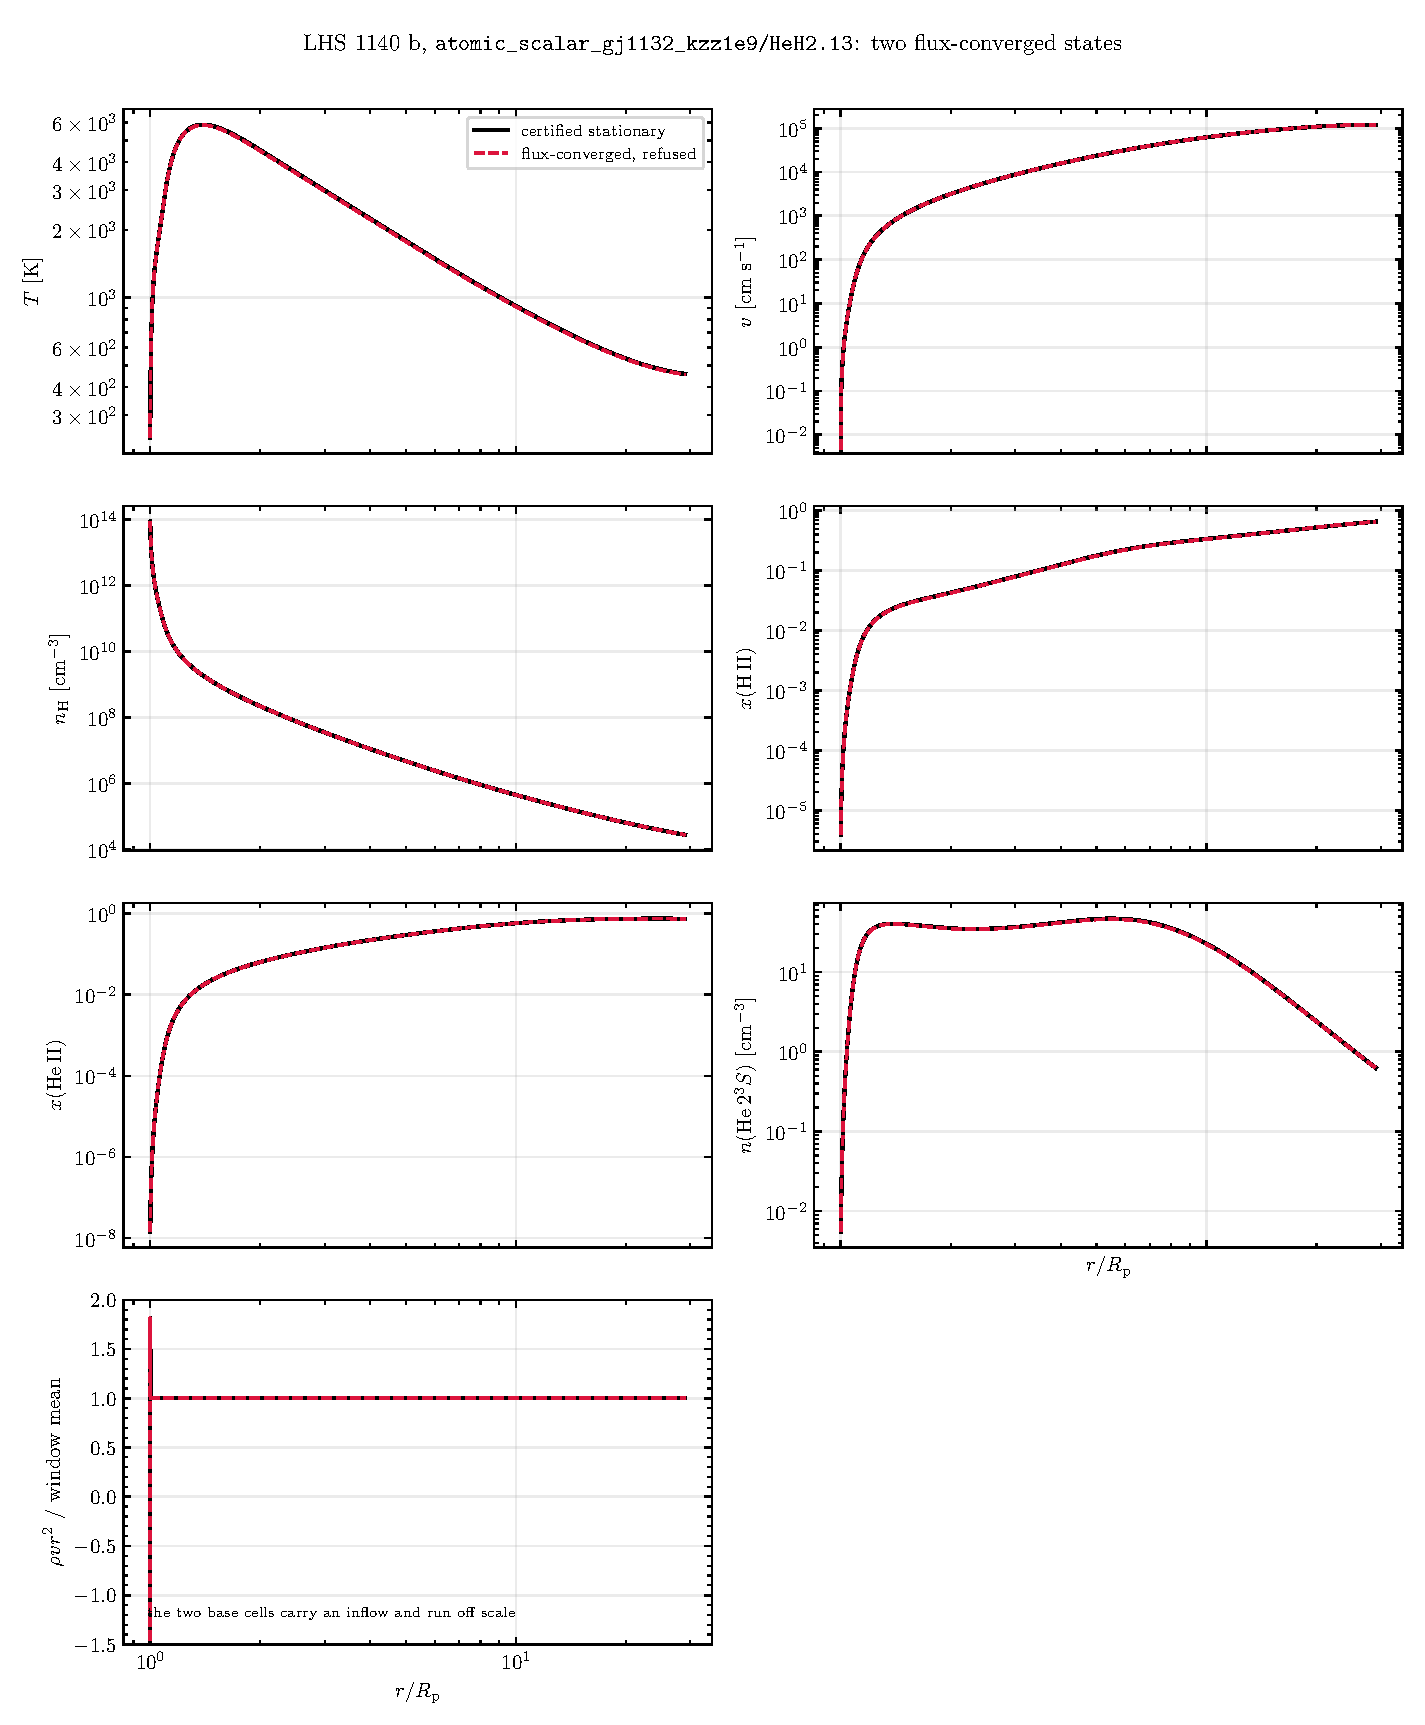
\includegraphics[width=\textwidth]{figures/du_stop_vs_stationary_profiles.pdf}
\caption{The certified stationary solution and the flux-converged refused
state of \texttt{scalar\_kzz1e9/HeH2.13}, as functions of radius.}
\end{figure}

\begin{figure}[htbp]
\centering
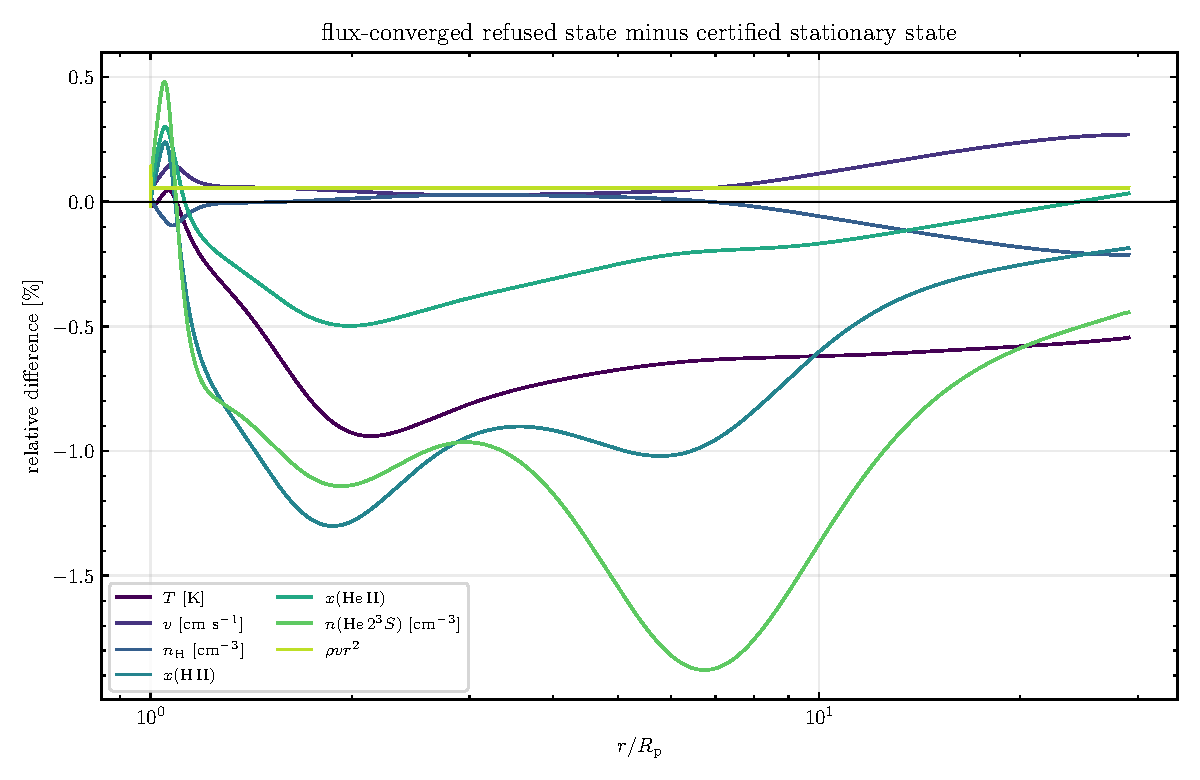
\includegraphics[width=\textwidth]{figures/du_stop_vs_stationary_differences.pdf}
\caption{The same two states, as the relative difference of each quantity.
The largest are the temperature at $r = 2.13\,R_p$ ($-0.94$ per cent),
$x(\mathrm{H\,II})$ at 1.87 ($-1.30$) and $n(\mathrm{He}\,2^3S)$ at 6.74
($-1.88$).}
\end{figure}

\begin{figure}[htbp]
\centering
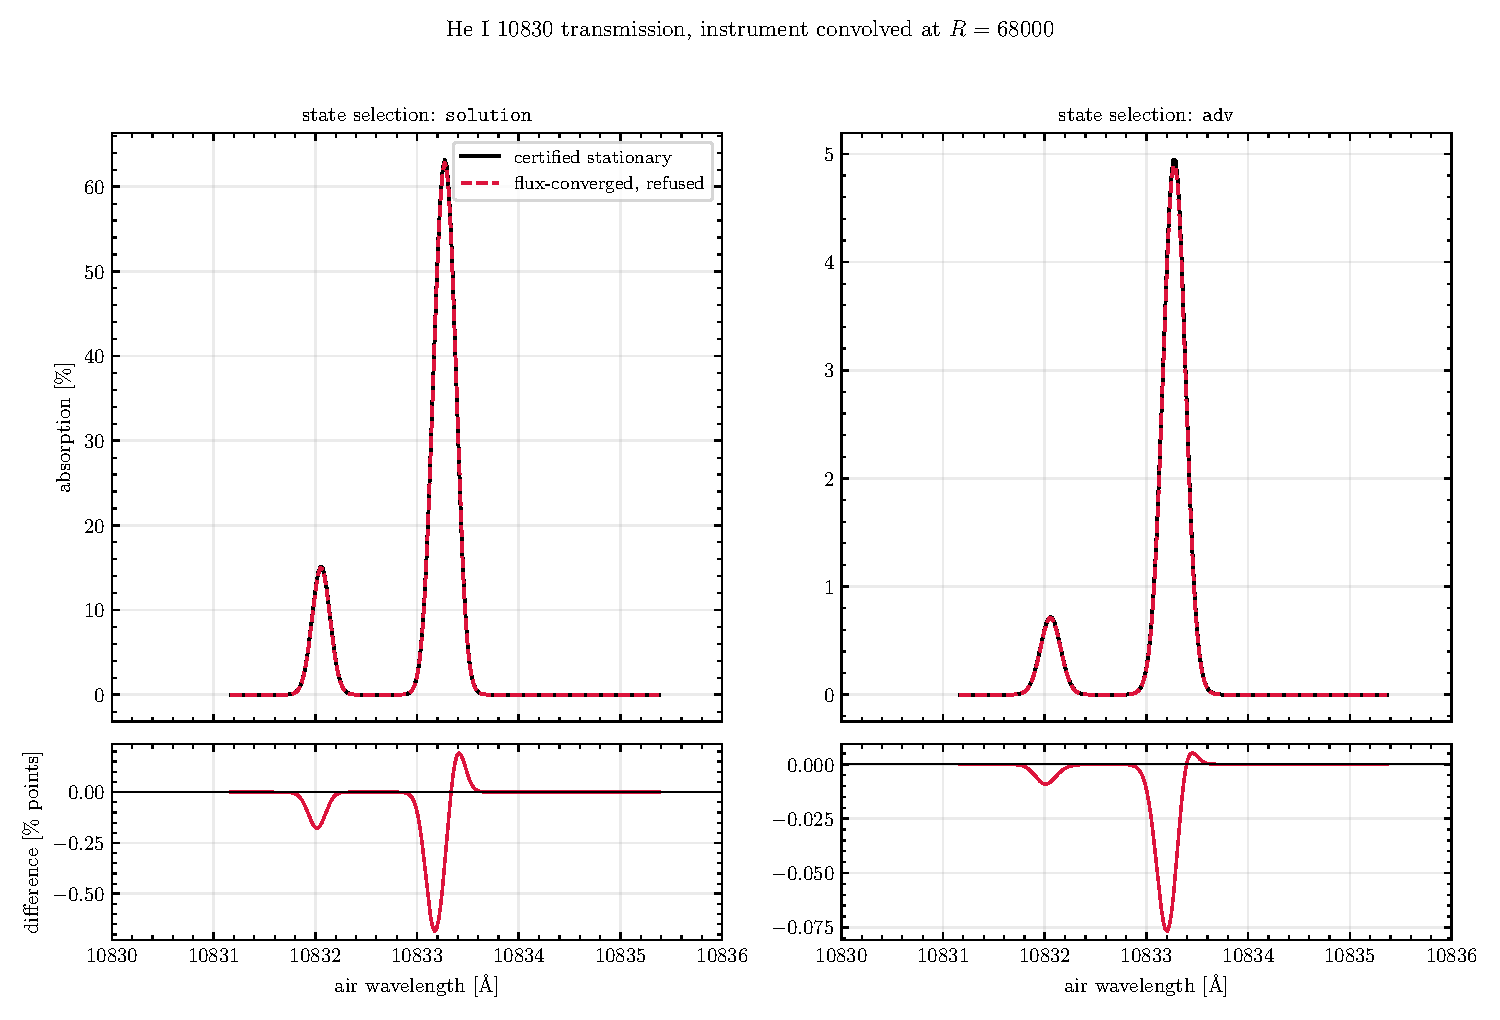
\includegraphics[width=0.85\textwidth]{figures/du_stop_vs_stationary_he10830.pdf}
\caption{The He~I 10830 transmission of the two states.}
\end{figure}

\end{document}
